\documentclass{article}
\usepackage[margin=1in]{geometry}
\usepackage{amsmath}
\usepackage{graphicx}
\usepackage{float}
\usepackage{listings}
\usepackage{xcolor}

\lstset{
    language=Matlab,
    basicstyle=\ttfamily\footnotesize,
    keywordstyle=\color{blue},
    breaklines=true
}

\begin{document}

\section*{Problem 2(a)}

The unsteady advection-diffusion problem is solved using linear finite elements in space ($E=100$, uniform) and a 3rd-order Backward Differentiation Formula with 3rd-order explicit extrapolation (BDF3/EXT3) in time. The diffusion term is treated implicitly, while the advection term is treated explicitly to avoid solving a non-symmetric system.

\subsection*{Time Integration Scheme}
The semi-discrete system is:
\begin{equation}
    B\underline{u}_t + cC\underline{u} = -\nu A\underline{u}
\end{equation}
The BDF3/EXT3 scheme requires bootstrapping the first two time steps. Let $\Delta t = 0.001$.
\begin{itemize}
    \item \textbf{Step 1 (BDF1/EXT1):} $\left(\frac{1}{\Delta t} B + \nu A\right) u^1 = \frac{1}{\Delta t} B u^0 - c C u^0$
    \item \textbf{Step 2 (BDF2/EXT2):} $\left(\frac{3}{2\Delta t} B + \nu A\right) u^2 = \frac{1}{\Delta t} B \left(2 u^1 - \frac{1}{2} u^0\right) - c C (2 u^1 - u^0)$
    \item \textbf{Step 3+ (BDF3/EXT3):} $\left(\frac{11}{6\Delta t} B + \nu A\right) u^{n+1} = \frac{1}{\Delta t} B \left(3 u^n - \frac{3}{2} u^{n-1} + \frac{1}{3} u^{n-2}\right) - c C (3 u^n - 3 u^{n-1} + u^{n-2})$
\end{itemize}

\subsection*{Results and Error Analysis}
The solution at $t=1.5$ is subjected to the Dirichlet boundary conditions $u(0,t) = \sin(\pi t)$ and $u(1,t) = 0$. 

Observing the wave profile, the primary numerical artifact is the presence of \textbf{trailing oscillations} behind the main wave. This is a symptom of \textbf{numerical dispersion} (phase error). Because standard Galerkin linear finite elements lack stabilization (such as upwinding), the higher-frequency components of the numerical solution travel at slower wave speeds than the exact physical speed, causing them to lag and form a dispersive tail.

\begin{figure}[H]
    \centering
    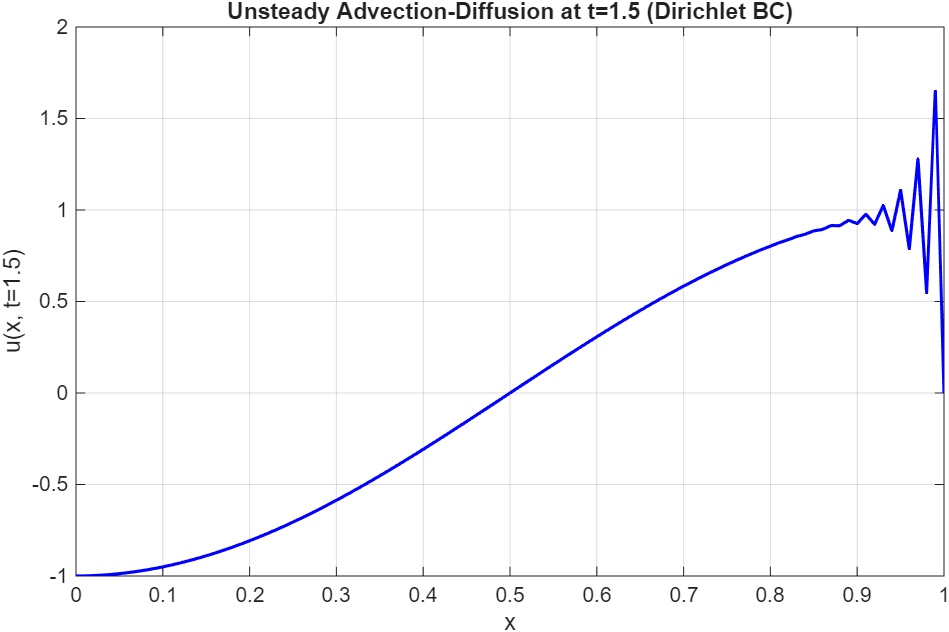
\includegraphics[width=0.7\textwidth]{2_a.png}
    \caption{Unsteady Advection-Diffusion at $t=1.5$ with Dirichlet BCs.}
    \label{fig:2a}
\end{figure}

\subsection*{MATLAB Implementation}
\begin{lstlisting}
L = 1.0; c = 1.0; nu = 1e-3; f = 0.0;
E = 100; N = E + 1; h = L / E;
dt = 0.001; t_end = 1.5;
n_steps = round(t_end / dt);

x = linspace(0, L, N)';
A = sparse(N, N); C = sparse(N, N); B = sparse(N, N);

for e = 1:E
    A_e = (1.0 / h) * [1.0, -1.0; -1.0, 1.0];
    C_e = 0.5 * [-1.0, 1.0; -1.0, 1.0];
    B_e = (h / 6.0) * [2.0, 1.0; 1.0, 2.0];
    
    idx = [e, e+1];
    A(idx, idx) = A(idx, idx) + A_e;
    C(idx, idx) = C(idx, idx) + C_e;
    B(idx, idx) = B(idx, idx) + B_e;
end

U = zeros(N, n_steps + 1);

LHS1 = (1/dt)*B + nu*A;
LHS2 = (3/(2*dt))*B + nu*A;
LHS3 = (11/(6*dt))*B + nu*A;

for n = 1:n_steps
    t_next = n * dt;
    
    if n == 1
        RHS = (1/dt)*B*U(:, n) - c*C*U(:, n);
        LHS = LHS1;
    elseif n == 2
        RHS = (1/dt)*B*(2*U(:, n) - 0.5*U(:, n-1)) - c*C*(2*U(:, n) - U(:, n-1));
        LHS = LHS2;
    else
        RHS = (1/dt)*B*(3*U(:, n) - 1.5*U(:, n-1) + (1/3)*U(:, n-2)) - ...
              c*C*(3*U(:, n) - 3*U(:, n-1) + U(:, n-2));
        LHS = LHS3;
    end
    
    LHS_bc = LHS;
    LHS_bc(1, :) = 0; LHS_bc(1, 1) = 1; RHS(1) = sin(pi * t_next);
    LHS_bc(end, :) = 0; LHS_bc(end, end) = 1; RHS(end) = 0;
    
    U(:, n+1) = LHS_bc \ RHS;
end
\end{lstlisting}

\end{document}